% =========================================================================
% Gemelo digital con SCADA 4.0 e IA para una celda de remachado e
% inspección de interruptores CAFI — Schneider Electric Challenge 3.0
% Formato IEEE Conference (IEEEtran). Compilar con pdfLaTeX + BibTeX
% (en Overleaf: subir la carpeta completa, compilador pdfLaTeX).
%
% Todos los datos técnicos de este documento fueron verificados contra el
% código de los repos RaspberryPiGIT y SchneiderProjectWeb_DigitalTwin
% (auditoría del 2026-08-18). La fidelidad de cada dato se etiqueta
% conforme a la Tabla de fidelidad (Sección de Resultados).
% =========================================================================
\documentclass[conference]{IEEEtran}
\IEEEoverridecommandlockouts

\usepackage[utf8]{inputenc}
\usepackage[T1]{fontenc}
\usepackage[spanish,es-tabla,es-noshorthands]{babel}
\usepackage{graphicx}
\usepackage{booktabs}
\usepackage{amsmath}
\usepackage{siunitx}
% siunitx v3 (Overleaf actual) eliminó \bar y hace opcional \byte:
\DeclareSIUnit\bar{bar}
\DeclareSIUnit\byte{B}
\usepackage{listings}
\usepackage{xcolor}
\usepackage{tikz}
\usetikzlibrary{arrows.meta,positioning}
\usepackage{cite}
\usepackage{hyperref}

\graphicspath{{figuras/}}

\lstset{basicstyle=\ttfamily\scriptsize, breaklines=true, frame=single,
        numbers=left, numberstyle=\tiny\color{gray}, captionpos=b}

\begin{document}

\title{Gemelo digital con SCADA 4.0 e inteligencia artificial para una celda
semi-automatizada de remachado e inspección de interruptores CAFI\\
{\footnotesize Schneider Electric Challenge 3.0 --- ITESM, Equipo 3}}

\author{
\IEEEauthorblockN{Enrique Amir González H.}
\IEEEauthorblockA{ITESM Campus Monterrey\\kiki7o@outlook.es}
\and
\IEEEauthorblockN{Diego Becerra Fuentes}
\IEEEauthorblockA{ITESM Campus Monterrey}
\and
\IEEEauthorblockN{Rodrigo Díaz Arrigunaga}
\IEEEauthorblockA{ITESM Campus Monterrey}
\and
\IEEEauthorblockN{Santiago Ordóñez Ramírez}
\IEEEauthorblockA{ITESM Campus Monterrey}
}

\maketitle

\begin{abstract}
Se presenta el diseño y la implementación de un gemelo digital con SCADA 4.0
e inteligencia artificial para una celda semi-automatizada de remachado e
inspección de interruptores miniatura con protección combinada de falla de
arco (CAFI), desarrollada para el Schneider Electric Challenge 3.0. Una
Raspberry Pi 4 actúa como \emph{gateway} IIoT y orquestador de facto de la
celda: adquiere la telemetría del cobot Lexium por Modbus TCP a 10 Hz (121
registros por muestreo), lo comanda mediante un protocolo TLS/JSON, integra
una cámara industrial Datalogic P15 por HTTP, opera el HMI físico como
maestro Modbus y acciona la mesa indexadora mediante GPIO, exponiendo el
conjunto a través de un backend FastAPI con un WebSocket de telemetría y 35
puntos de acceso REST. El gemelo digital, accesible desde el navegador
(React Native Web, three.js y urdf-loader), replica la celda con modelos
URDF y anima el cobot con telemetría real; sobre él, una capa SCADA 4.0
aporta analítica en cinco pilares ---detección de anomalías por z-score y
seguridad, mantenimiento predictivo, optimización de proceso y soporte de
decisiones SOP--- junto con un copiloto de mantenimiento basado en un
modelo de lenguaje. Se documenta
el contraste entre la arquitectura PLC-céntrica propuesta y la
implementación gateway-céntrica resultante, se etiqueta explícitamente la
fidelidad de cada dato (telemetría real, derivado, simulación o
demostración) y se discuten las lecciones de integrar equipo industrial
heterogéneo con hardware de bajo costo.
\end{abstract}

\begin{IEEEkeywords}
gemelo digital, SCADA, Industria 4.0, cobot, Modbus TCP, IIoT, visión
artificial, Raspberry Pi
\end{IEEEkeywords}

% =========================================================================
\section{Introducción}
El ensamble final de un interruptor termomagnético requiere remachar su
carcasa e inspeccionar el resultado. En la estación de trabajo que motiva
este proyecto, dicho proceso es manual: el operador toma la pieza de una
canaleta, la coloca en un \emph{fixture} dentro de una cabina, acciona un
mando bimanual, inspecciona visualmente los remaches y registra el resultado
en una lista de verificación en papel, con un tiempo aproximado de cinco
minutos por pieza. El proceso presenta puntos de pellizco al colocar la
pieza, riesgo de aplastamiento dentro de la cabina y error humano en una
inspección subjetiva.

En el marco del \emph{Schneider Electric Challenge 3.0} (ITESM Campus
Monterrey, 2026) se planteó diseñar, validar y construir un prototipo de
baja resolución de un sistema mecatrónico semi-automatizado que inspeccione
y automatice el remachado del producto CAFI utilizando el cobot Lexium de
Schneider Electric \cite{lexiumcobot}, con tres ejes rectores: seguridad
(eliminar pellizco y aplastamiento), calidad (inspección automática de los
cinco remaches con resultado en el HMI) y eficiencia. El producto de
referencia es el interruptor Square~D Homeline HOM120PCAFI
\cite{hom120pcafi} (\SI{120}{\volt}~CA, \SI{20}{\ampere}, \SI{277}{\gram}),
replicado para el prototipo mediante impresión 3D con cinco marcadores que
simulan los remaches.

Este artículo documenta el sistema construido y, en particular, su gemelo
digital. Las contribuciones son:
\begin{enumerate}
  \item Un \emph{gateway} IIoT de bajo costo (Raspberry Pi 4) que integra
        cinco protocolos heterogéneos (Modbus TCP, TLS/JSON, HTTP, FTP y
        GPIO) y orquesta el ciclo completo de la celda, asumiendo el rol de
        controlador central que el diseño original asignaba a un PLC.
  \item Un gemelo digital accesible desde el navegador que replica la celda
        con modelos URDF y anima el cobot con telemetría real a 10 Hz,
        distinguiendo siempre entre datos reales, derivados, simulados y de
        demostración.
  \item Una capa SCADA 4.0 con cinco pilares de analítica heurística
        sobre señales reales y un copiloto de mantenimiento basado en un
        modelo de lenguaje con respaldo local sin conexión.
  \item Un sistema de inspección por visión que verifica los cinco remaches
        del CAFI integrando una cámara industrial mediante su interfaz HTTP.
  \item Un análisis del contraste entre la arquitectura PLC-céntrica
        propuesta y la implementación gateway-céntrica final, con las
        lecciones aprendidas de la integración.
\end{enumerate}

% =========================================================================
\section{Marco teórico y trabajo relacionado}
El concepto de gemelo digital, formalizado por Grieves y Vickers
\cite{grieves2017digital}, designa una réplica virtual de un sistema físico
sincronizada con éste durante su ciclo de vida. Tao \emph{et al.}
\cite{tao2019digital} revisan su adopción industrial y señalan la
convergencia entre gemelos digitales, IoT industrial y analítica de datos.
Kritzinger \emph{et al.} \cite{kritzinger2018digital} proponen una
clasificación según el grado de integración de datos: \emph{modelo digital}
(sin intercambio automático), \emph{sombra digital} (flujo automático solo
del físico al virtual) y \emph{gemelo digital} (flujo bidireccional). Bajo
esa taxonomía, el sistema aquí descrito opera como sombra digital en su
modo de visualización (telemetría en un solo sentido a 10 Hz) y alcanza la
categoría de gemelo cuando se habilitan los comandos de control remoto
(movimiento articular, mesa, banda e inspección) desde la interfaz web.

Lee \emph{et al.} \cite{lee2015cyber} estructuran los sistemas ciberfísicos
para Industria 4.0 en la arquitectura de cinco niveles 5C
(conexión, conversión, ciber, cognición y configuración). La celda descrita
cubre los niveles de conexión y conversión en el \emph{gateway}, el nivel
ciber en el gemelo web y el nivel de cognición en la capa SCADA 4.0 con
analítica; el nivel de configuración (reconfiguración autónoma del proceso)
queda como trabajo futuro.

En cuanto a los protocolos, la telemetría del cobot se adquiere con Modbus
TCP \cite{modbus2012,modbustcp2006}, el estándar de facto para integración con equipo
industrial heredado, mientras que el diseño original preveía la
programación del control en un PLC conforme a IEC 61131-3 \cite{iec61131} y
la interoperabilidad futura mediante OPC UA \cite{iec62541}. La seguridad de
la celda se enmarca en las normas de robótica industrial ISO 10218-1/-2
\cite{iso10218-1,iso10218-2} y en la especificación de robots colaborativos
ISO/TS 15066 \cite{isots15066}, cuyo contenido fue incorporado a las
ediciones 2025 de ISO 10218.

% =========================================================================
\section{Contexto del reto y proceso objetivo}
El alcance acordado con Schneider Electric incluyó la integración del cobot
Lexium con un PLC Modicon M262 \cite{modiconM262} y un HMI, el mecanismo de
inspección, los prototipos de CAFI y \emph{fixtures} por manufactura aditiva
(PLA/PETG con insertos metálicos) y la validación experimental. Quedaron
fuera del alcance la remachadora industrial operativa ---el remachado se
representa mediante un ciclo simulado de \SI{30}{\second}---, el despliegue a
gran escala y la certificación comercial.

El efector final es un gripper de tres dedos con mecanismo de pantógrafo
accionado por un cilindro neumático de doble efecto MAL16$\times$25 (émbolo
de \SI{16}{\milli\metre}, carrera de \SI{25}{\milli\metre}, presión máxima
de \SI{6}{\bar}): la extensión abre los dedos y la retracción los cierra. El
criterio de calidad es binario: una pieza con los cinco remaches detectados
PASA; con menos de cinco, NO PASA, y el resultado se refleja en el HMI. La
validación del reto contempló ambas pruebas (pieza correcta y pieza
defectuosa). El diseño de seguridad se apoyó en ANSI/RIA R15.06,
ISO 10218 \cite{iso10218-1,iso10218-2}, ISO/TS 15066 \cite{isots15066} e
ISO 12100,
con guarda física alrededor de la cabina y verificación de zona libre antes
de cada ciclo.

% =========================================================================
\section{Arquitectura del sistema}
El hallazgo central de este trabajo es la coexistencia de dos arquitecturas
del mismo sistema: la propuesta (PLC-céntrica) y la implementada
(gateway-céntrica). La Tabla~\ref{tab:comparativa} las contrasta componente
a componente.

\subsection{Arquitectura propuesta (PLC-céntrica)}
El diseño presentado al inicio del reto define once componentes: HMI de
7 pulgadas, PLC Modicon M262 como controlador central, cobot Lexium,
gripper neumático, canaleta de alimentación pasiva, \emph{fixture} de
remachado con dos pistones neumáticos de sujeción, \emph{fixture} de
inspección, sistema de visión, pistón de rechazo, canasta de rechazo y punto
de estiba final. El PLC orquesta la secuencia completa, gestiona las señales
de seguridad y comunica resultados al HMI; la comunicación troncal es
EtherNet/IP y el operador interactúa únicamente con el HMI.

\subsection{Arquitectura implementada (gateway-céntrica)}
En la práctica, una Raspberry Pi 4 sustituyó al PLC como orquestador
(Fig.~\ref{fig:arquitectura}). La tarjeta es \emph{dual-homed}: participa en
la subred industrial (192.168.1.0/24, donde residen la cámara, el HMI y el
PLC previsto) y en la subred del cobot (10.5.5.0/24), y además enruta entre
ambas mediante NAT (\texttt{iptables MASQUERADE}). Sobre ella corre un
backend FastAPI \cite{fastapi} que habla directamente con cada dispositivo:
Modbus TCP con el cobot (lectura) y con el HMI (como maestro), TLS/JSON con
el controlador del cobot (comandos), HTTP con la cámara, FTP para programas
del robot y GPIO para la mesa indexadora, la banda y los sensores de los
\emph{fixtures} (Tabla~\ref{tab:protocolos}). El PLC Modicon TM262-15
(192.168.1.50) y el servidor OPC UA de EcoStruxure (192.168.1.201:4840)
quedaron documentados en la arquitectura implementada como ``integración
futura'', sin participación activa en el ciclo.

\begin{figure}[t]
  \centering
  \begin{tikzpicture}[
    font=\scriptsize,
    capa/.style={draw, rounded corners=2pt, align=center,
                 text width=0.86\columnwidth, inner sep=5pt},
    enlace/.style={{Stealth[length=2mm]}-{Stealth[length=2mm]}, thick},
    node distance=5.5mm
  ]
    \node[capa, fill=gray!12] (web) {\textbf{Capa 4 --- Gemelo digital web}\\
      Expo / React Native Web + three.js + urdf-loader\\
      7 vistas, 6 idiomas, SCADA 4.0 + IA (PaaS + Caddy)};
    \node[capa, fill=gray!4, below=of web] (tunel)
      {\textbf{Capa 3 --- Túnel público}\\
      WSS/HTTPS con dominio estático (ngrok)};
    \node[capa, fill=gray!12, below=of tunel] (rpi)
      {\textbf{Capa 2 --- Gateway IIoT (Raspberry Pi 4)}\\
      FastAPI :8000 $\cdot$ orquestador del ciclo (32 pasos)\\
      maestro Modbus del HMI $\cdot$ GPIO $\cdot$ NAT dual-red};
    \node[capa, fill=gray!4, below=of rpi] (planta)
      {\textbf{Capa 1 --- Planta física}\\
      Cobot Lexium (Modbus TCP $\cdot$ TLS/JSON $\cdot$ FTP)\\
      Cámara Datalogic P15 (HTTP) $\cdot$ HMI Schneider (Modbus TCP)\\
      Mesa indexadora + banda + sensores (GPIO)};
    \draw[enlace] (web) -- node[right]{WebSocket JSON a 10 Hz + REST} (tunel);
    \draw[enlace] (tunel) -- (rpi);
    \draw[enlace] (rpi) -- node[right]{5 protocolos} (planta);
  \end{tikzpicture}
  \caption{Arquitectura de cuatro capas del sistema implementado. La
  Raspberry Pi 4 orquesta la planta y sirve la telemetría al gemelo web a
  través de un túnel TLS con dominio estático.}
  \label{fig:arquitectura}
\end{figure}

\begin{table}[t]
  \caption{Protocolos integrados por el gateway IIoT.}
  \label{tab:protocolos}
  \centering
  \scriptsize
  \begin{tabular}{@{}llll@{}}
    \toprule
    Dispositivo & Protocolo & Puerto & Función \\
    \midrule
    Cobot Lexium & Modbus TCP (FC04) & 6502 & Telemetría a 10 Hz \\
    Cobot Lexium & TLS/JSON & 10001 & Comandos de movimiento y E/S \\
    Cobot Lexium & TLS/JSON & 10000 & Estado en tiempo real \\
    Cobot Lexium & FTP (TLS) & 2121 & Programas \texttt{.jks} \\
    Cámara P15 & HTTP & 80 & Captura e inspección \\
    HMI Schneider & Modbus TCP (esclavo) & 502 & LEDs, botones, contadores \\
    Mesa, banda, sensores & GPIO & --- & Actuación y detección local \\
    Navegador & WSS/HTTPS & 443 & Gemelo digital \\
    \bottomrule
  \end{tabular}
\end{table}

\begin{table*}[t]
  \caption{Contraste entre la arquitectura propuesta y la implementada.}
  \label{tab:comparativa}
  \centering
  \scriptsize
  \begin{tabular}{@{}p{0.14\textwidth}p{0.36\textwidth}p{0.40\textwidth}@{}}
    \toprule
    Función & Propuesta (PLC-céntrica) & Implementada (gateway-céntrica) \\
    \midrule
    Orquestador & PLC Modicon M262 vía EtherNet/IP & Raspberry Pi 4 con FastAPI; máquina de estados de 32 pasos en Python \\
    PLC & Cerebro central del sistema & TM262-15 presente en red (192.168.1.50) pero sin integración activa; ``integración futura'' \\
    Interoperabilidad & EtherNet/IP troncal & Modbus TCP, TLS/JSON, HTTP, FTP y GPIO hablados directamente por el gateway; OPC UA diferido \\
    Cobot & ``Lexium Cobot'' comandado por el PLC & Lexium LXMRL03S0000 (6 GDL, \SI{3}{\kilo\gram}, alcance \SI{626}{\milli\metre}) con 4 canales simultáneos hacia la RPi \\
    HMI & Par del PLC vía EtherNet/IP & Esclavo Modbus TCP de la RPi: 15 LEDs (bobinas 1--15), 6 botones (101--106), 4 registros \\
    Alimentación & Canaleta pasiva & Banda transportadora motorizada (DO13) con sensor fotoeléctrico \\
    Sujeción/rechazo & Pistones neumáticos comandados por PLC & Clasificación por trayectoria del cobot a contenedores de aceptadas/rechazadas \\
    Inspección & ``Sistema de visión'' genérico & Datalogic P15 (1.3 MP monocromática) integrada por HTTP; algoritmo propio de 5 remaches \\
    Gemelo digital & No contemplado & Aplicación web completa con URDF, telemetría en vivo y SCADA 4.0 + IA \\
    Redes & Una red implícita & Dos subredes con NAT en la RPi; túnel TLS de dominio estático para el acceso público \\
    \bottomrule
  \end{tabular}
\end{table*}

% =========================================================================
\section{El gateway IIoT}

\subsection{Adquisición de telemetría por Modbus TCP}
El lector Modbus muestrea el controlador del cobot cada \SI{100}{\milli\second}
(función FC04, \emph{Read Input Registers}, unidad 1, puerto 6502) leyendo
121 registros en 12 bloques por instantánea; los valores FLOAT32 e INT32 se
decodifican en \emph{big-endian} con la palabra alta primero. La
Tabla~\ref{tab:modbus} resume el mapa. El backend agrega a cada instantánea
el estado de la mesa, sensores, gripper, ciclo y métricas, y la difunde por
el WebSocket \texttt{/ws/cobot} a 10 Hz; además expone 35 puntos de acceso
REST (\texttt{/api/cobot/*}, \texttt{/api/table/*}, \texttt{/api/camera/*},
\texttt{/api/cycle/*}, \texttt{/api/pipeline/*}).

\begin{table}[t]
  \caption{Mapa de registros Modbus del cobot Lexium (FC04), verificado en
  el código del lector.}
  \label{tab:modbus}
  \centering
  \scriptsize
  \begin{tabular}{@{}lll@{}}
    \toprule
    Registros & Contenido & Tipo \\
    \midrule
    316--327 & Temperaturas de junta (6) & INT32 \\
    340--357 & Error / habilitación / colisión por junta & UINT16 \\
    358--369 & Corrientes de junta (6) & FLOAT32 \\
    370--381 & Fuerza y par del efector ($F_{x,y,z}$, $T_{x,y,z}$) & FLOAT32 \\
    382--393 & Posiciones de junta [\si{\degree}] & FLOAT32 \\
    394--405 & Velocidades de junta [\si{\degree\per\second}] & FLOAT32 \\
    406--417 & Pose TCP $(X,Y,Z,R_x,R_y,R_z)$ & FLOAT32 \\
    418--429 & Velocidades del TCP & FLOAT32 \\
    454--461 & Estado (paro protectivo, e-stop, potencia, \ldots) & UINT16 \\
    462--465 & Velocidad global [\%]; código de error & F32/I32 \\
    466--471 & Controlador: temperatura, potencia, corriente & FLOAT32 \\
    \bottomrule
  \end{tabular}
\end{table}

\subsection{Control del cobot}
Los comandos viajan por un canal TLS/JSON al puerto 10001 del controlador
(protocolo nativo del fabricante del brazo), previa activación del modo
\emph{Remote Control} en EcoStruxure Cobot Expert; sin ella, el controlador
responde \texttt{permission deny}. Un hallazgo de integración relevante:
en el firmware instalado el comando de movimiento cartesiano \texttt{moveL}
se acepta (código de error 0) pero nunca se ejecuta. El
\emph{gateway} lo resuelve con un puente de cinemática inversa: solicita
\texttt{kine\_inverse} al propio controlador, verifica la solución con
\texttt{kine\_forward} (tolerancia de ida y vuelta $\leq$
\SI{3}{\milli\metre} y salto articular $\leq$ \SI{55}{\degree}) y ejecuta un
\texttt{joint\_move} articular. Un segundo hallazgo: sondear las entradas
digitales a 10 Hz por el mismo puerto que comparte EcoStruxure provocaba la
autodeshabilitación del robot, por lo que el sondeo se limitó a 5 Hz.
Como el robot también se deshabilita por inactividad aceptando comandos sin
ejecutarlos, cada movimiento va precedido de una verificación de
habilitación contra la telemetría Modbus.

\subsection{Orquestación del ciclo}
El ciclo de producción de una pieza es una secuencia determinista de 32
pasos (Fig.~\ref{fig:ciclo}): tras el pre-vuelo (energizado y habilitación)
y el \emph{homing} de la mesa, la banda avanza hasta que el sensor
fotoeléctrico detecta un CAFI; el cobot lo toma, lo coloca en el
\emph{fixture} de remachado, la mesa indexa hacia la posición de remachado
(una rotación de \SI{180}{\degree} en el modelo cinemático de la celda) y
permanece \SI{30}{\second} (ciclo de remachado simulado, sin actuador
comandado), regresa, y el cobot lleva la pieza a la placa de visión; tras
una espera de inspección de hasta \SI{5}{\second}, el veredicto PASS/FAIL
determina el contenedor destino y el brazo regresa a HOME. La biblioteca de
poses contiene 25 posturas articulares definidas en grados de controlador
más 5 poses altas de aproximación (desplazamientos en $Z$ de $+65$ a
$+150$ \si{\milli\metre}) cuyos valores articulares se cargan desde un
archivo de ajustes externo al repositorio; la velocidad por defecto es
15\,\% y cada movimiento tiene un tiempo límite de \SI{30}{\second}.

Sobre la misma base existe un \emph{pipeline} concurrente multi-pieza
(hasta 20 CAFIs, 8 por defecto) gobernado por un planificador puro de siete
rangos de prioridad (completar colocación en curso $>$ retirar pieza
inspeccionada $>$ gestión de cámara ocupada $>$ tomar de banda $>$ retirar
remachada $>$ rotar mesa $>$ reposo), con oportunismo de cámara y
enclavamientos que impiden rotar la mesa con el cobot en su zona. La banda
y la rotación corren como tareas de fondo concurrentes y la corrida termina
sola tras \SI{30}{\second} sin piezas nuevas. En modo de apilado, las
piezas se estiban por capas de \SI{25}{\milli\metre} (máximo 10) usando el
puente de cinemática inversa descrito.

\begin{figure}[t]
  \centering
  \begin{tikzpicture}[
    font=\scriptsize,
    paso/.style={draw, rounded corners=2pt, align=center,
                 text width=0.62\columnwidth, inner sep=3pt},
    fin/.style={draw, rounded corners=2pt, align=center,
                text width=0.27\columnwidth, inner sep=3pt},
    flecha/.style={-{Stealth[length=2mm]}, thick},
    node distance=3.2mm
  ]
    \node[paso, fill=gray!8]  (p1) {1. Pre-vuelo y \emph{homing} de mesa (pasos 0--2)};
    \node[paso, below=of p1]  (p2) {2. Banda hasta sensor fotoeléctrico; pick del CAFI (3--6)};
    \node[paso, fill=gray!8, below=of p2] (p3) {3. Colocación en \emph{fixture} de remachado (7--11)};
    \node[paso, below=of p3]  (p4) {4. Indexado \SI{180}{\degree} + remachado \SI{30}{\second} + retorno (12--13)};
    \node[paso, fill=gray!8, below=of p4] (p5) {5. Retiro de pieza remachada (14--16)};
    \node[paso, below=of p5]  (p6) {6. Colocación en placa de visión; inspección $\leq$ \SI{5}{\second} (17--23)};
    \node[paso, fill=gray!8, below=of p6] (p7) {7. Retiro de placa y tránsito a contenedores (24--27)};
    \node[fin, below=5mm of p7, xshift=-0.16\columnwidth, fill=green!8]  (ok) {PASS $\rightarrow$ contenedor de aceptadas};
    \node[fin, below=5mm of p7, xshift=0.16\columnwidth, fill=red!8] (ko) {FAIL $\rightarrow$ contenedor de rechazadas};
    \node[paso, below=18mm of p7] (p9) {8. Retorno seguro a HOME (31--32)};
    \draw[flecha] (p1) -- (p2);
    \draw[flecha] (p2) -- (p3);
    \draw[flecha] (p3) -- (p4);
    \draw[flecha] (p4) -- (p5);
    \draw[flecha] (p5) -- (p6);
    \draw[flecha] (p6) -- (p7);
    \draw[flecha] (p7.south) -- (ok.north);
    \draw[flecha] (p7.south) -- (ko.north);
    \draw[flecha] (ok.south) -- (p9.west |- ok.south) -- (p9.170);
    \draw[flecha] (ko.south) -- (p9.east |- ko.south) -- (p9.10);
  \end{tikzpicture}
  \caption{Ciclo secuencial de 32 pasos ejecutado por el gateway (entre
  paréntesis, los índices de paso publicados en la telemetría). El
  remachado es un ciclo simulado de \SI{30}{\second} conforme al alcance
  del reto.}
  \label{fig:ciclo}
\end{figure}

\subsection{Integración del HMI físico}
El HMI Schneider funciona como esclavo Modbus TCP (192.168.1.51:502) y la
RPi como maestro con un lazo de \SI{200}{\milli\second}: escribe 15 LEDs en
las bobinas 1--15 (incluido el semáforo rojo/ámbar/verde), tres contadores
de producción (total, aceptadas, rechazadas) y un registro con el estado de
la cámara, y lee seis botones en las bobinas 101--106 (START, STOP, RESUME,
RESTART, CONFIRM\_CLEAN, FINALIZE) con detección de flanco. Así, el operador
de planta conserva un punto de mando físico aunque el orquestador sea el
\emph{gateway}.

\subsection{Actuación local por GPIO}
La mesa indexadora se desplaza entre dos finales de carrera accionada por
un motor a pasos (STEP en GPIO17, DIR en GPIO27, límites en GPIO22/23); no
hay codificador, por lo que la posición se conoce únicamente por los
límites (el modelo cinemático de la celda representa este recorrido como
una rotación de \SI{180}{\degree}). El perfil de velocidad es trapezoidal (aceleración de 166 a
417 pasos/s en 250 pasos y arrastre final a 143 pasos/s hasta asentar el
final de carrera), con recorridos medidos de 497 a 821 pasos y un tiempo de
indexado de 3.2 a \SI{4.0}{\second} en banco. El generador de pasos corre en
un subproceso dedicado para aislarlo de las pausas del intérprete del
backend. Dos microinterruptores en GPIO24/25 detectan la presencia de pieza
en los \emph{fixtures}.

% =========================================================================
\section{El gemelo digital web}

\subsection{Pila tecnológica y modelo 3D}
La aplicación se construyó con Expo SDK 52 / React Native Web 0.19 y
TypeScript 5.9 en modo estricto; el render 3D usa three.js 0.170
\cite{threejs} con react-three-fiber 8.18 y el cargador URDF de NASA JPL
\cite{urdfloaders}. Ofrece siete vistas (inicio, diagrama de cableado
interactivo generado desde el DXF original, celda 3D simulada, cobot en
vivo, lógica de planta, SCADA y SCADA de simulación), control de acceso por
roles (ADMIN, DEMO y OPERATOR) y seis idiomas. El modelo del robot es un
URDF con seis juntas de revolución más una prismática para el gripper
(carrera de 0 a \SI{28}{\milli\metre}); la celda completa (mesa de
$2.0\times\SI{1.6}{\metre}$, banda, mesa indexadora, cabina de remachado,
estación de visión y contenedores) proviene de un paquete
URDF/Xacro derivado del CAD, con 124 mallas STL (\SI{21.8}{\mega\byte} de
activos estáticos en total). El
despliegue es estático: la exportación web se sirve con Caddy en una
plataforma PaaS, y el navegador alcanza el backend de la celda mediante un
túnel TLS con dominio estático, necesario porque una página HTTPS no puede
abrir WebSockets sin cifrar hacia la LAN.

\subsection{Telemetría y fidelidad de datos}
La vista ``Cobot en vivo'' anima el URDF con las posiciones articulares
reales aplicando la transformación de convención controlador$\to$modelo
\begin{equation}
  \theta_i^{\mathrm{URDF}} = s_i\,\theta_i^{\mathrm{ctrl}} + o_i,
  \label{eq:transform}
\end{equation}
con $s = (1,-1,1,1,1,1)$ y $o = (-90, 90, 0, -90, 0, 0)$ grados, y suaviza
el render con easing exponencial. La misma transformación inversa convierte
las poses del modelo en comandos articulares reales. La interfaz distingue
cuatro modos (\emph{live} con datos Modbus por WebSocket,
\emph{connecting}, \emph{demo} con una instantánea real pregrabada, y
\emph{error}) más un estado derivado, \emph{backend demo}, cuando el
gateway responde pero el cobot está fuera de línea (bandera presente en
cada trama); los mandos de control solo se habilitan en modo \emph{live} y
los datos se marcan obsoletos tras \SI{3}{\second} sin tramas.
Como el \emph{gateway} no publica el ángulo de la mesa en tiempo real, la
vista lo reconstruye entre los dos finales de carrera a $\pi/4$ rad/s; este
dato es derivado, no medido.

\subsection{Máquina de estados de la celda y validación}
La vista de celda 3D no depende de la planta: la gobierna una máquina de
estados finitos pura y determinista que modela banda, mesa con dos
\emph{fixtures}, remachadora (\SI{30}{\second} exactos), visión y cobot como
recurso único con planificador de prioridades, hasta dos piezas en cola y
enclavamiento anticolisión mesa-cobot. El tipo de estado distingue 6 estados
de celda, 15 estados por pieza y 10 tareas del cobot, con 9 eventos de
operador (incluido FINALIZE, que drena el trabajo en proceso, a diferencia
de STOP). Diecisiete pruebas unitarias cubren el ciclo completo con
veredictos PASS y FAIL, la concurrencia de dos piezas, la cola llena, la
recuperación por RESTART con limpieza confirmada y el reinicio seguro.

% =========================================================================
\section{Inspección por visión}
La cámara Datalogic P15 \cite{datalogicP15} (CMOS monocromático de
$1280\times1024$) se integró mediante su interfaz HTTP con la secuencia
\emph{offline} $\to$ captura PNG $\to$ \emph{online}. El algoritmo de
inspección, propio del proyecto, primero registra la imagen a un marco
canónico de $436\times651$ píxeles (umbralización, componentes conexas,
rectificación por rectángulo de área mínima, resolución del volteo de
\SI{180}{\degree} por correlación con plantilla y refinamiento afín) y
después evalúa cinco regiones de interés, una por remache, mediante
contraste local: un remache presente produce un hueco oscuro de área
$\geq 481$ píxeles, mientras que la marca de un remache faltante ronda los
110 ---una separación de ${\approx}4.4\times$ entre clases---, por lo que
el umbral de decisión de 250 píxeles conserva márgenes de
${\approx}1.9\times$ y ${\approx}2.3\times$ hacia cada clase (calibrado con
muestras reales). El
veredicto es PASS si y solo si se detectan los cinco remaches
(Fig.~\ref{fig:inspeccion}); cualquier error de captura o registro se trata
como FAIL, favoreciendo los falsos rechazos sobre los falsos aceptados.

\begin{figure}[t]
  \centering
  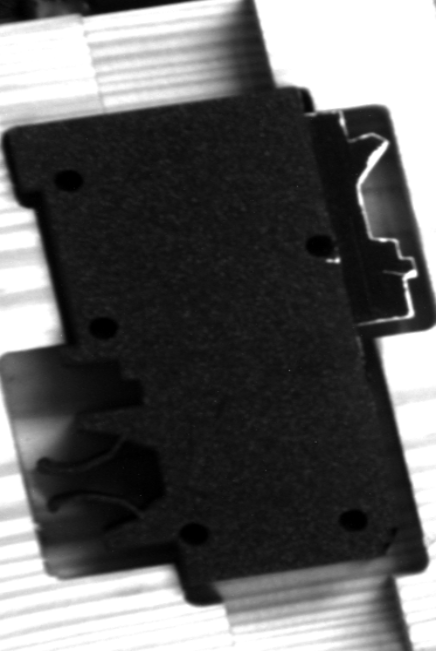
\includegraphics[width=0.72\columnwidth]{camara_cafi_template}
  \caption{Plantilla de referencia de la inspección: captura real de la
  cámara Datalogic P15 ($1280\times1024$, monocromática) del CAFI en el
  \emph{fixture} de visión; se aprecian los orificios de los cinco puntos
  de remache evaluados. [Telemetría real.]}
  \label{fig:inspeccion}
\end{figure}

% =========================================================================
\section{SCADA 4.0 con inteligencia artificial}

\subsection{Motor SCADA y alarmas}
La vista SCADA abre su propia conexión de solo lectura al \emph{gateway} y
sigue una política \emph{real-only}: toda señal sin fuente real se muestra
como no disponible en lugar de simularse, y cada dato lleva su procedencia
(real, obsoleto, no conectado o demo). El motor itera a 4 Hz sobre una
matriz canónica de 14 entradas y 8 salidas, mantiene un historial acotado
(120 puntos a 1 Hz) y gestiona alarmas con ciclo de vida
activa/reconocida/resuelta que no pueden cerrarse mientras la condición
persista. La Tabla~\ref{tab:umbrales} resume los umbrales. Al no existir un
bloque de fase publicado por el PLC, la etapa del ciclo se infiere de las
señales con un esquema de prioridades de 10 etapas, y el tiempo de ciclo
real se cronometra por flancos (válido entre 5 y \SI{600}{\second}).

\begin{table}[t]
  \caption{Umbrales de alarma y de analítica del SCADA (verificados en la
  configuración del código).}
  \label{tab:umbrales}
  \centering
  \scriptsize
  \begin{tabular}{@{}lll@{}}
    \toprule
    Señal & Advertencia & Alarma / crítico \\
    \midrule
    Temperatura de junta & $>\SI{50}{\celsius}$ & $>\SI{60}{\celsius}$ / $>\SI{70}{\celsius}$ \\
    Fuerza en el efector & $>\SI{20}{\newton}$ & $>\SI{40}{\newton}$ \\
    Banda encendida & $>\SI{60}{\second}$ & $>\SI{120}{\second}$ \\
    Presión del gripper & $<\SI{5.5}{\bar}$ & $<\SI{5.0}{\bar}$ \\
    Anomalía (z-score) & $|z|>2.0$ & $|z|>3.0$ \\
    Vida útil restante (RUL) & $<25\,\%$ & $<8\,\%$ \\
    Vibración (proxy: $\sigma$ de corrientes) & $>\SI{0.6}{\ampere}$ & $>\SI{1.2}{\ampere}$ \\
    Variabilidad de ciclo (CV) & $>0.18$ & --- \\
    Datos obsoletos & $>\SI{3}{\second}$ & --- \\
    Piezas en planta & --- & $>8$ \\
    \bottomrule
  \end{tabular}
\end{table}

\subsection{Los cinco pilares de analítica}
La capa de IA cubre los cinco pilares del proyecto con cuatro módulos
heurísticos deterministas que se derivan en cada iteración sobre señales
reales ---la detección de anomalías y la seguridad industrial comparten
módulo---, sin modelos entrenados y con la regla explícita de no inventar
valores ausentes, más un copiloto de mantenimiento que opera bajo demanda:
\begin{itemize}
  \item \textbf{Detección de anomalías y seguridad} (\emph{The Watchman}):
        z-score del último valor contra la media y desviación estándar de la
        serie previa (mínimo 5 muestras) sobre cuatro series ---tiempo de
        ciclo, temperatura del controlador, tiempo de banda encendida y
        temperatura articular máxima---, combinado con las banderas de
        seguridad del cobot (e-stop, paro protectivo, colisión, error de
        movimiento).
  \item \textbf{Mantenimiento predictivo} (\emph{The Mechanic}): vida útil
        restante lineal del actuador de remachado sobre una vida nominal de
        50\,000 ciclos; proxy de vibración por dispersión de las corrientes
        articulares; tendencia térmica por regresión de mínimos cuadrados; y
        estabilidad del proceso por coeficiente de variación del tiempo de
        ciclo.
  \item \textbf{Optimización} (\emph{The Optimizer}): rendimiento
        (piezas/hora), porcentaje de inactividad respecto de los
        \SI{35}{\second} de trabajo útil (remachado más inspección), energía
        por ciclo estimada, y una recomendación de consigna de velocidad
        (objetivo 85\,\%, penalizada ante variabilidad alta o juntas
        calientes, acotada a 50--100\,\%) que nunca se aplica sola al
        hardware.
  \item \textbf{Soporte de decisiones} (\emph{The Coordinator}): traduce el
        veredicto transversal a CONTINUAR / RETENER / PARAR con
        procedimientos operativos estándar y pasos de recuperación por
        categoría de falla; PARAR se reserva a fallas de seguridad o
        hardware.
  \item \textbf{Copiloto de mantenimiento}: ante una alarma, la interfaz
        envía el contexto (solo datos reales, con la lista explícita de
        señales no disponibles) a un servicio de diagnóstico externo a los
        repositorios auditados ---declarado en la documentación del
        proyecto--- que consulta un modelo de lenguaje; si no responde en
        \SI{8}{\second}, un diagnóstico heurístico local, que es la parte
        verificada en código, toma su lugar, y la respuesta se etiqueta
        visiblemente según su origen (IA o respaldo local).
\end{itemize}

\subsection{Trazabilidad de piezas}
Como la planta no emite identificadores de pieza, un rastreador los infiere
por flancos: cada activación del sensor fotoeléctrico crea una pieza nueva y
las etapas (10 por pieza) se atribuyen por orden de llegada; el ciclo cierra
con el flanco del veredicto de cámara. El SCADA de simulación, en cambio,
registra la trazabilidad exacta (marcas de tiempo de cada hito por pieza) y
exporta cada corrida como CSV de cuatro secciones y JSON con la analítica
incluida.

% =========================================================================
\section{Resultados y validación}
\label{sec:resultados}

\subsection{Etiquetado de fidelidad}
Siguiendo la práctica recomendada para gemelos digitales, todo dato del
sistema (y de este artículo) pertenece a una de las clases de la
Tabla~\ref{tab:fidelidad}; la interfaz las señala con insignias visibles.
La Fig.~\ref{fig:scadaoffline} ilustra la política \emph{real-only} en su
caso extremo: con el \emph{gateway} fuera de línea, el SCADA muestra cada
indicador como no disponible en lugar de rellenarlo con valores sintéticos.

\begin{figure}[t]
  \centering
  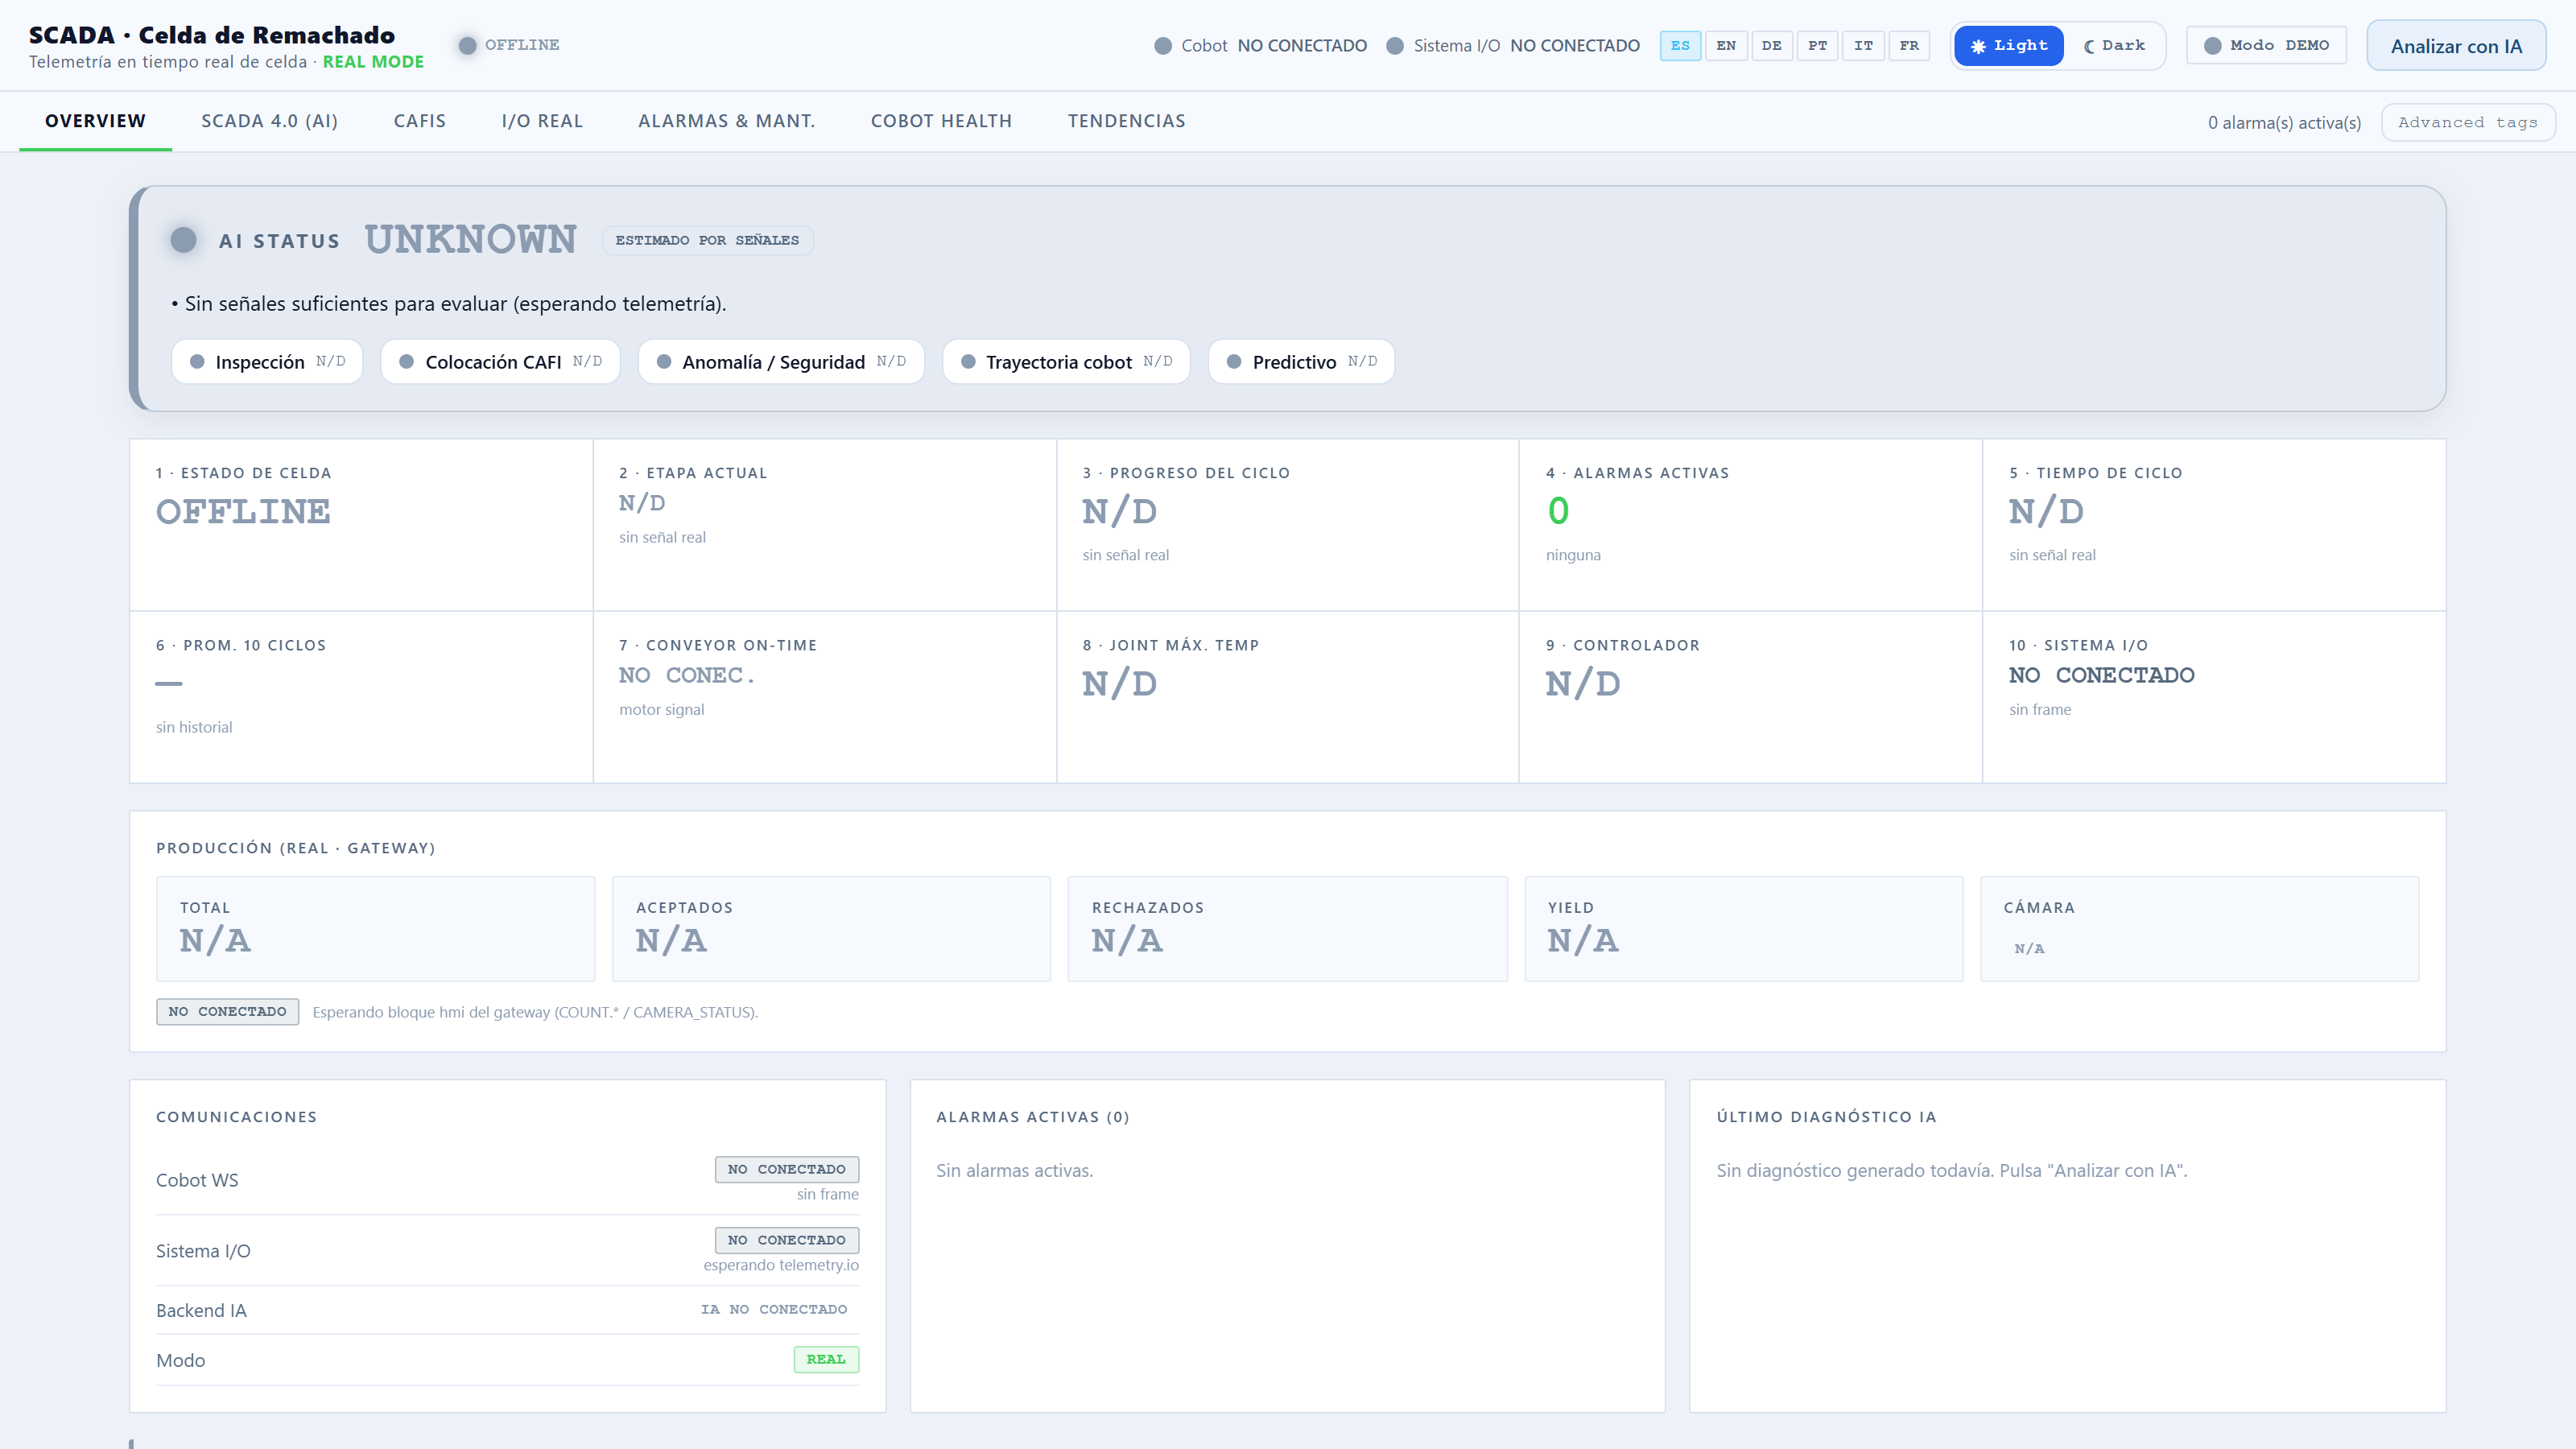
\includegraphics[width=\columnwidth]{captura_scada_offline}
  \caption{Panel SCADA en modo real con el \emph{gateway} fuera de línea:
  la política \emph{real-only} muestra cada señal sin fuente como
  N/D en lugar de simularla, y los canales de comunicación reportan su
  estado. [Telemetría real ausente, honestamente señalada.]}
  \label{fig:scadaoffline}
\end{figure}

\begin{table}[t]
  \caption{Clases de fidelidad de los datos del sistema.}
  \label{tab:fidelidad}
  \centering
  \scriptsize
  \begin{tabular}{@{}lp{0.62\columnwidth}@{}}
    \toprule
    Clase & Descripción y ejemplos \\
    \midrule
    Telemetría real & Lecturas Modbus del cobot físico, sensores GPIO, capturas de la cámara P15. \\
    Derivado & Etapa de ciclo inferida por prioridades de señales; ángulo de mesa reconstruido entre finales de carrera; identificadores de pieza por flancos. \\
    Simulación local & Máquina de estados de la celda 3D y SCADA de simulación (sin red). \\
    Demostración & Instantánea real pregrabada usada como respaldo sin conexión, siempre marcada con bandera \texttt{demo}. \\
    \bottomrule
  \end{tabular}
\end{table}

\subsection{Validación funcional}
Con la clasificación anterior, lo verificado es lo siguiente.
\emph{Sobre el hardware real}: la cadena completa de telemetría (cobot
$\to$ Modbus $\to$ WebSocket $\to$ URDF en el navegador) está implementada
a 10 Hz y fue operada sobre el cobot físico, con instantáneas reales
conservadas en los repositorios (mayo--junio de 2026); el control remoto de
movimiento quedó registrado en la bitácora del \emph{gateway} (junta 1
desplazada de \SI{0}{\degree} a \SI{45}{\degree} y \SI{90}{\degree} por
TLS/JSON, mayo de 2026); la biblioteca de poses articulares fue capturada
en el robot físico (junio de 2026); la mesa indexó entre límites en
3.2--\SI{4.0}{\second} de forma repetible en banco; y el algoritmo de
visión se calibró con piezas reales, con una separación de
${\approx}4.4\times$ entre las áreas de remache presente ($\geq 481$ px) y
faltante ($\approx 110$ px) alrededor del umbral de 250 px. La inspección
satisface el criterio del reto: pieza con 5 remaches $\to$ PASA; con menos
$\to$ NO PASA. \emph{En simulación}: la máquina de estados cuenta con 17
pruebas unitarias que cubren su comportamiento completo, y el planificador
concurrente fue validado en corridas en seco de 1, 2, 3, 5 y 10 piezas con
cero violaciones de enclavamiento.

Dos limitaciones de medición deben declararse: el repositorio no registra
tiempos de ciclo de producción medidos en corridas físicas completas (las
métricas de tiempo de ciclo existen como instrumentación, no como conjunto
de datos), y los indicadores de ocupación del cobot solo son alimentados por
el simulador. Asimismo, el remachado es un ciclo temporizado de
\SI{30}{\second} sin actuador comandado, conforme al alcance del reto.

\begin{figure}[t]
  \centering
  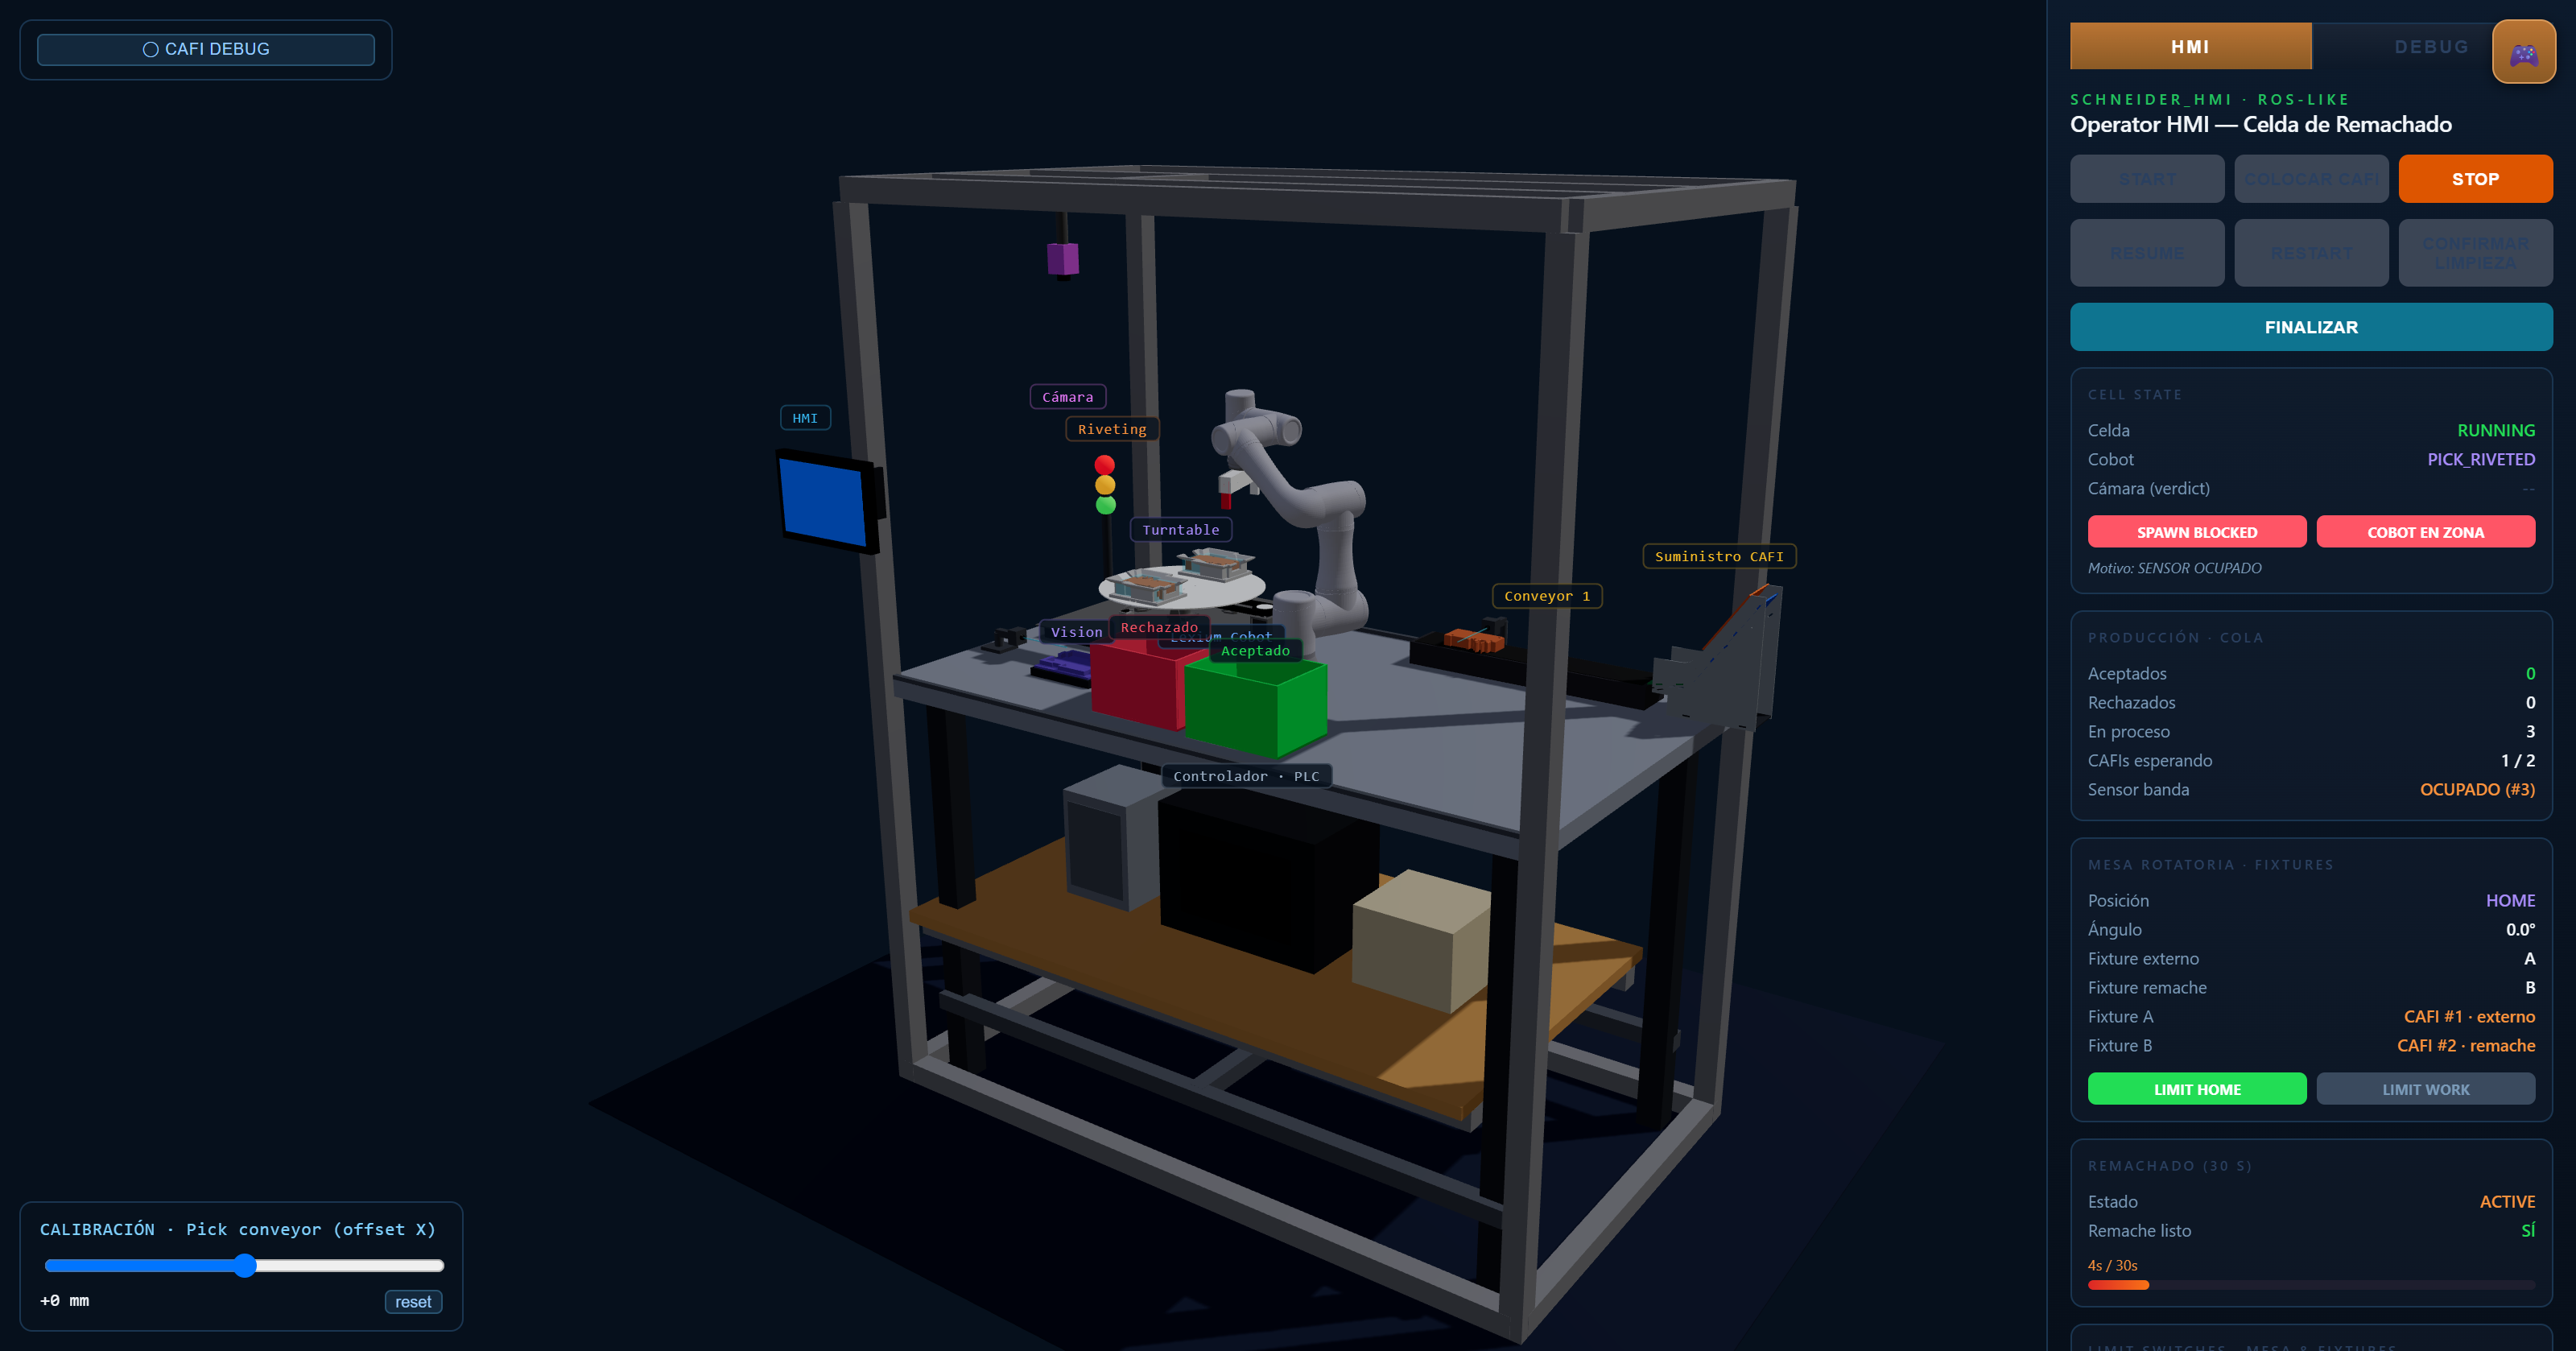
\includegraphics[width=\columnwidth]{captura_visor3d}
  \caption{Vista ``Celda 3D'' del gemelo digital: modelo URDF de la celda
  completa gobernado por la máquina de estados local. A la derecha, el HMI
  de operador con la celda en RUNNING, piezas en ambos \emph{fixtures},
  el temporizador de remachado activo (\SI{30}{\second}) y los
  enclavamientos visibles (\emph{spawn} bloqueado, cobot en zona).
  [Simulación local.]}
  \label{fig:visor}
\end{figure}

\begin{figure}[t]
  \centering
  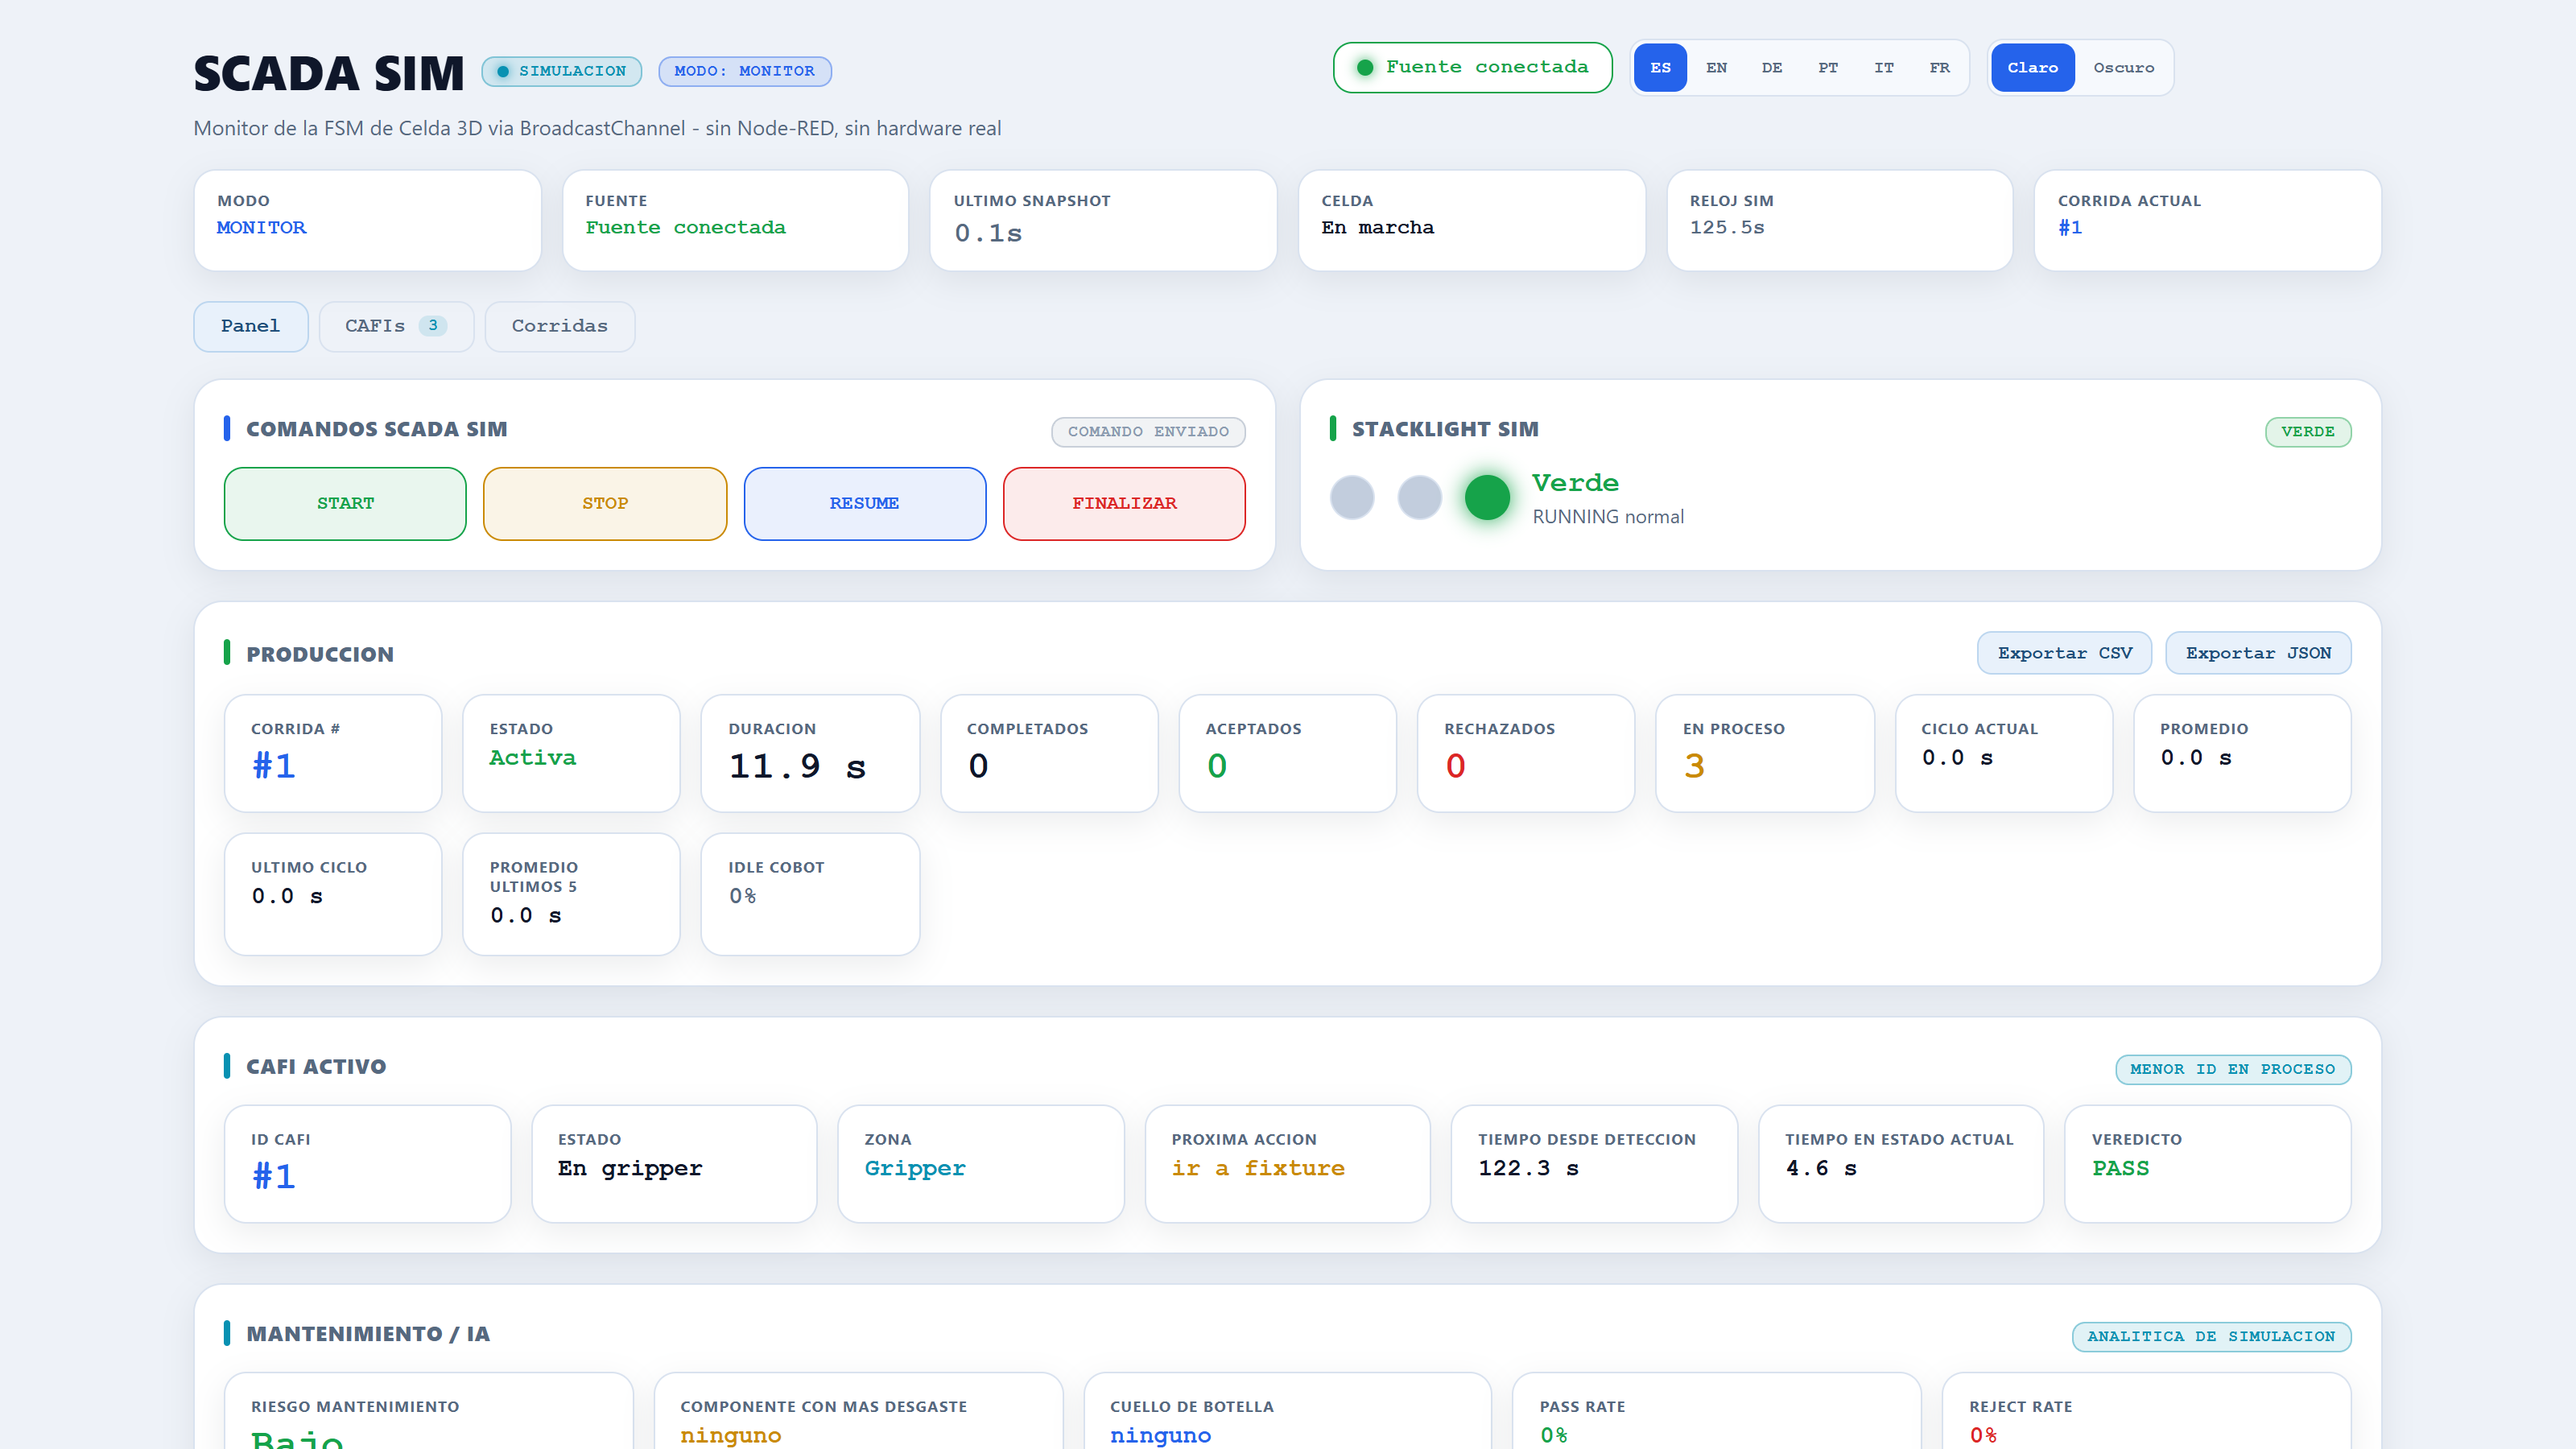
\includegraphics[width=\columnwidth]{captura_scadasim}
  \caption{SCADA de simulación local, alimentado por la máquina de estados
  de la celda 3D mediante \emph{BroadcastChannel} (sin red): corrida activa
  con tres piezas en proceso, semáforo virtual y trazabilidad de la pieza
  activa con su veredicto. [Simulación local.]}
  \label{fig:scadasim}
\end{figure}

% =========================================================================
\section{Discusión}
La divergencia entre las dos arquitecturas no fue una decisión de pizarrón
sino el resultado acumulado de restricciones prácticas: el PLC no llegó a
integrarse en el plazo del reto; el canal de comandos del cobot resultó
tener limitaciones no documentadas (el \texttt{moveL} inerte, la
autodeshabilitación al sondear a 10 Hz, la dependencia del modo
\emph{Remote Control}); y el equipo necesitaba una superficie de
programación rápida para iterar. Un \emph{gateway} en Python con protocolos
abiertos ofreció esa superficie y, de paso, hizo trivial exponer la
telemetría como JSON para el gemelo web, algo que una arquitectura
EtherNet/IP pura habría requerido pasarelas adicionales. El costo de esa
flexibilidad es real y debe nombrarse: el orquestador no es un controlador
industrial endurecido ni certificado, y la cadena de seguridad física
(paro de emergencia cableado al orquestador) quedó pendiente ---el
\emph{gateway} solo observa los estados de paro del propio cobot---, con la
guarda física y las paradas del robot como salvaguardas vigentes.

Otras limitaciones conocidas: el túnel de dominio estático es un punto
único de falla y deja el backend expuesto, con CORS abierto y sin
autenticación, por lo que la única mitigación es operativa (mantener el
túnel activo solo durante las sesiones de trabajo); la autenticación de la
aplicación web reside en el cliente;
la interfaz Telnet de la cámara carece de autenticación de fábrica; y la
validación de la concurrencia multi-pieza es, hasta ahora, en seco. Nada de
esto invalida la tesis central, pero acota su alcance a entornos educativos
y de prototipado.

La lección generalizable es doble. Primero, un gemelo digital útil no
requiere la pila de integración canónica: con un \emph{gateway} de bajo
costo que normalice protocolos heterogéneos a JSON sobre WebSocket, la capa
de visualización y analítica se vuelve tecnología web estándar. Segundo, la
disciplina de etiquetar la fidelidad de cada dato (real, derivado, simulado,
demo) ---adoptada aquí desde el diseño--- es lo que permite que un sistema
con partes simuladas siga siendo honesto como herramienta de ingeniería, en
línea con la distinción modelo/sombra/gemelo de
\cite{kritzinger2018digital}.

% =========================================================================
\section{Conclusiones y trabajo futuro}
Se construyó y documentó una celda semi-automatizada de remachado e
inspección de interruptores CAFI con un gemelo digital web completo: un
\emph{gateway} IIoT que orquesta cinco protocolos y un ciclo de 32 pasos,
telemetría real a 10 Hz animando un modelo URDF en el navegador, inspección
por visión de los cinco remaches con margen de decisión calibrado, y una
capa SCADA 4.0 con cinco pilares de analítica y copiloto de mantenimiento.
El contraste documentado entre el diseño PLC-céntrico y la implementación
gateway-céntrica constituye, más que una desviación, un caso de estudio de
integración pragmática en Industria 4.0.

El trabajo futuro sigue el orden inverso de las limitaciones: (1) integrar
el PLC Modicon TM262-15 y el servidor OPC UA \cite{iec62541} ya presentes en
la red, migrando hacia ellos las funciones de seguridad y control de bajo
nivel; (2) cablear la cadena de paro de emergencia física al arranque del
ciclo (la compuerta de software ya existe y está deliberadamente sin
conectar); (3) endurecer el acceso (autenticación en el backend y en la
aplicación); (4) medir y publicar los indicadores de producción reales
(tiempos de ciclo físicos, OEE) que la instrumentación ya soporta; y (5)
sustituir gradualmente las heurísticas de los pilares por modelos entrenados
con los históricos que el propio SCADA acumula.

\section*{Agradecimientos}
Los autores agradecen a Schneider Electric por el planteamiento del reto y
el acceso al equipo Lexium, Modicon y Harmony, y al Tecnológico de Monterrey
por la infraestructura del laboratorio y la asesoría durante el
Schneider Electric Challenge 3.0.

\bibliographystyle{IEEEtran}
\bibliography{referencias}

\end{document}
